\documentclass[handouts]{beamer}
\usepackage[orientation=portrait,size=a4, scale=2]{beamerposter}
\beamertemplatenavigationsymbolsempty

\usepackage[czech]{babel}
\usepackage{booktabs}

\title{Model metapopulací}
\author{Robert Mařík}
\usetheme{CambridgeUS}
\usecolortheme{crane}

\def\subsection#1{\par\medskip \textbf{#1}\par\medskip}
\begin{document}

\begin{frame}

  \vskip 0 pt plus 1 filll
  
  \begin{center}
    \large Model metapopulací
  \end{center}

  \vskip 0 pt plus 1 filll

  Americký ekolog Richard Levins představil v roce 1969 model \textbf{metapopulací}. Jedná se o populace žijící ve fragmentovaném prostředí, které je možno studovat jako systém oddělených populací, které spolu komunikují díky možnosti migrace.

    \begin{itemize}
    \item Uvažujme populaci žijící ve fragmentovaném prostředí. Tuto
      fragmentaci si můžeme představit jako systém ostrůvků, ve
      kterých se populace nachází. Tyto ostrůvky (fragmenty) jsou
      zřetelně odděleny. (Například louky nebo lesní palouky.)
    \item 
Některé z těchto podlokalit (fragmentů) mohou být nevhodné pro trvalé osídlení a populace na nich může přežívat jen díky přistěhovalcům.
\item 
Na některých podlokalitách zase může vlivem náhodných jevů populace zcela vymřít a za několik let se zde může znovu objevit, díky přenesení několika jedinců z jiné podlokality, kteří se zde rozmnoží.
\item 
Předpokládejme, že míra migrace je tak malá, že není možné posuzovat populaci jako jedinou populaci, která se řídí logistickou nebo jinou obdobnou rovnicí. Taková síť místních malých populací, které jsou propojeny občasnými náhodnými migracemi, se nazývá metapopulace.
\end{itemize}

  
\begin{columns}
  \begin{column}{0.47\hsize}
\begin{block}{Model metapopulace (Levins)}
  \begin{itemize}
  \item Označme $P$ procento obsazených fragmentů. Změna tohoto počtu
    za jednotku času je rozdílem nově osídlených fragmentů a
    fragmentů, na kterých populace vymizela. 
  \item Rychlost osidlování
    nových fragmentů souvisí s počtem obsazených fragmentů, ze kterých
    populace přeskočí na nově osídlenou lokalitu a s počtem volných
    fragmentů.
  \item Rychlost vymírání souvisí s počtem osídlených fragmentů.
  \item Předpokládejme, že všechny závislosti jsou modelovány přímou úměrností. Model má potom tvar $$\frac{\mathrm dP}{\mathrm dt}=k P (1-P) - mP.$$
\end{itemize}
\end{block}
\end{column}
\begin{column}{0.47\hsize}
\begin{block}{Modifikace modelu metapopulací}

\begin{itemize}
\item \textbf{Propagační déšť.} Pokud jsou fragmenty blízko lokality, odkud mohou být osidlovány, nehraje v rychlosti osidlování roli počet osídlených populací. Model má potom tvar $$\frac{\mathrm dP}{\mathrm dt}=k (1-P) - mP.$$
\item \textbf{Záchranný efekt.} Pokud je obsazeno více fragmentů, mohou se tyto fragmenty stát zdrojem živočichů, kteří migrují i na lokalitu, kde by jinak populace vymřela. To sníží rychlost vymírání. Model má potom tvar
  $$\frac{\mathrm dP}{\mathrm dt}=k P (1-P) - mP(1-P).$$
\end{itemize}
\end{block}
\end{column}

\end{columns}
\vskip 0 pt plus 1 filll
%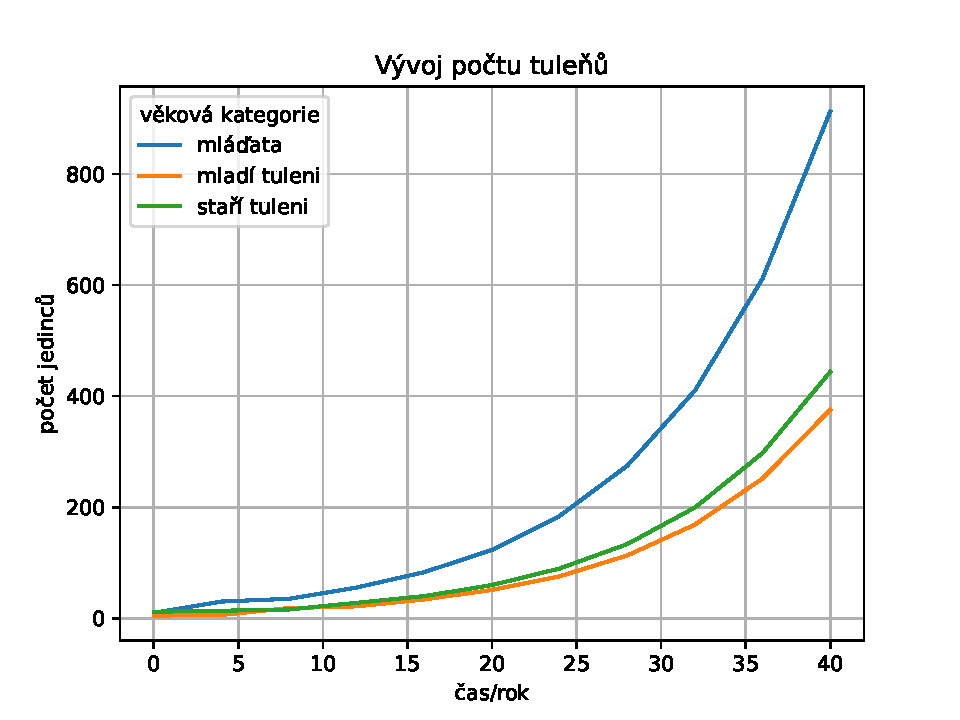
\includegraphics{tuleni.pdf}
\includegraphics[width=.48\linewidth]{metapopulace.pdf}%
\includegraphics[width=.48\linewidth]{metapopulace2.pdf}

\end{frame}
\end{document}


%%% Local Variables: 
%%% TeX-command-extra-options: "-shell-escape"
%%% TeX-engine: xetex
%%% End:
